%
% File acl2024.tex
%
%% Based on the style files for ACL 2023, which were
%% Based on the style files for ACL 2022, which were
%% Based on the style files for ACL 2021, which were
%% Based on the style files for ACL 2020, which were
%% Based on the style files for ACL 2019, which were based on ACL 2018, NAACL 2018, ACL 2017, ACL 2016, ACL 2015, ACL 2014, ACL 2013
%% Based on the style files for EACL 2009 and We use the official ACL class

\documentclass[11pt]{article}
\usepackage[T1]{fontenc}
\usepackage[utf8]{inputenc}
\usepackage{acl}
\usepackage{times}
\usepackage{latexsym}
\usepackage{graphicx}
\usepackage{booktabs}
\usepackage{multirow}
\usepackage{array}
\usepackage{tabularx}

\newcommand\BibTeX{B\textsc{ib}\TeX}

\title{Leakage-Aware Privacy-Practice Classification: A Comparative Study of Classical and Neural Models under Policy-Disjoint Evaluation}

\author{%
\begin{tabular}{cc}
Nafiz Ahmed Nafi & Priom Halder \\
{\small\normalfont\texttt{nafiz.ahmed.nafi@g.bracu.ac.bd}} &
{\small\normalfont\texttt{priom.halder@g.bracu.ac.bd}} \\[0.6em]
MD. Amirul Islam Sadat & Samiha Tasnim Orthi \\
{\small\normalfont\texttt{amirul.islam.sadat@g.bracu.ac.bd}} &
{\small\normalfont\texttt{samiha.tasnim.orthi@g.bracu.ac.bd}} \\[0.8em]
\multicolumn{2}{c}{\normalfont Department of Computer Science and Engineering, BRAC University}
\end{tabular}%
}

\begin{document}

\maketitle

\begin{abstract}
Privacy policies govern how personal data is collected, shared, and retained, yet most users never read them in full. We study automatic classification of annotated privacy-policy spans into eight data-practice categories using the OPP-115 corpus (17,343 labeled spans, 115 policies). TF-IDF is used for completed classical experiments; a Word2Vec pipeline was implemented but not executed for completed downstream classification. Models span three classical approaches (Random Forest, Logistic Regression, Naive Bayes) and seven neural architectures (SimpleRNN, GRU, LSTM, their bidirectional variants, and partially fine-tuned BERT Base). Our central contribution is systematic comparison of two evaluation protocols: conventional row-level stratified split and policy-disjoint split that holds entire policies out of training. Because privacy policies reuse boilerplate language, the row-level split inflates macro-F1 by 0.015--0.123 depending on model and changes apparent ranking. Under honest policy-disjoint evaluation, BERT Base achieves highest macro-F1 (0.706), narrowly ahead of Naive Bayes (0.701), showing smallest evaluation-protocol gap. Results suggest document-grouped evaluation should be standard for text classification tasks built on corpora with reused or template-based language.
\end{abstract}

\section{Introduction}

Privacy policies are the main legal instrument through which organizations disclose how they collect, use, share, and retain personal data. In practice, they are long, formulaically written, inconsistently structured, and surveys of user behavior repeatedly find that almost nobody reads one in full before consenting~\cite{mcdonald-cranor-2008-cost}. Automatically mapping policy text onto a standardized taxonomy of data practices would enable downstream tools to summarize policies at a glance, flag GDPR or CCPA-relevant language, or allow researchers to compare practices at corpus scale. This is a multi-class text classification problem and not a saturated task: privacy language is technical, class frequencies are heavily skewed, and single clauses often express more than one practice simultaneously.

We build our study on the OPP-115 corpus~\cite{wilson-etal-2016-creation}, containing 115 real-world website privacy policies annotated by legal experts against a fixed schema of data-practice categories. We treat each annotated span as one classification instance labeled with one of eight practice categories.

A less obvious property of this corpus motivates the paper's central contribution. Privacy policies reuse legally vetted boilerplate language across unrelated organizations---template clauses drafted by the same law firm recur verbatim across dozens of policies. A conventional row-level train/test split ignores this structure and can place near-identical boilerplate on both sides, letting a model score well by recognizing memorized phrases rather than by learning what privacy language of a given category actually looks like. This is an instance of the broader evaluation-leakage problem documented in NLP~\cite{gorman-bedrick-2019-need, lewis-etal-2021-question}.

\subsection{Research Questions}

\begin{itemize}
\item \textbf{RQ1:} How does a conventional row-level split change measured performance relative to a policy-disjoint split for the same model?
\item \textbf{RQ2:} How does this evaluation-protocol gap vary across classical, recurrent, and transformer architectures?
\item \textbf{RQ3:} Which model achieves the best macro-F1 on entirely unseen policies?
\end{itemize}

\subsection{Contributions}

\begin{enumerate}
\item A leakage-aware evaluation framework contrasting row-level and policy-disjoint splits across ten models spanning four architecture families.
\item An empirical finding that the evaluation-protocol gap varies substantially across model families.
\item Full implementation of the required classical and neural suite, with implementation gaps documented openly rather than omitted.
\end{enumerate}

Context-aware modeling, imbalance-aware training, and external validation are left for future work.

\section{Related Work}

\subsection{Privacy-Policy NLP}

The OPP-115 corpus~\cite{wilson-etal-2016-creation} is the standard manually annotated benchmark for data-practice classification in privacy policies.\ \citet{harkous-etal-2018-polisis} present Polisis, a deep-learning pipeline that classifies policy segments and supports downstream question answering, establishing that neural models can substantially outperform earlier rule-based approaches. Our work differs in focus: rather than proposing a new architecture, we study how the evaluation protocol specifically—whether the split respects document-level structure—changes which architecture appears to win.

\subsection{Classification Models}

TF-IDF paired with classical classifiers remains a strong, fast baseline~\cite{pedregosa-etal-2011-scikit}. Word embeddings such as Word2Vec~\cite{mikolov-etal-2013-efficient} and GloVe~\cite{pennington-etal-2014-glove} enable generalization across related terms. Recurrent architectures including LSTM~\cite{hochreiter-schmidhuber-1997-lstm}, GRU~\cite{cho-etal-2014-learning}, and their bidirectional variants~\cite{schuster-paliwal-1997-bidirectional} model sequential dependencies that bag-of-words representations discard. BERT~\cite{devlin-etal-2019-bert} adds contextual representations from large external corpora before task-specific fine-tuning.

\subsection{Evaluation Leakage and Class Imbalance}

\citet{gorman-bedrick-2019-need} show that re-splitting standard NLP benchmarks changes both absolute scores and relative rankings.\ \citet{lewis-etal-2021-question} document a related failure in question answering where train/test overlap inflates reported accuracy. Our work applies this principle---splits must respect data grouping structure---to a domain where that structure is unusually explicit.\ \citet{johnson-khoshgoftaar-2019-survey} survey class-imbalance mitigations; we adopt macro-F1 as the primary metric and include class-weighted configurations throughout.

\section{Methodology}

\subsection{Dataset and Exploratory Data Analysis}

\subsubsection{Corpus Description}

We use the OPP-115 corpus~\cite{wilson-etal-2016-creation}: 115 website privacy policies, each annotated by three annotators against a fixed schema, later merged at 0.75 overlap-similarity threshold that reproduces the corpus's own 92/23 policy train/test split. We take the longest populated selected span as the classification input and attach its surrounding clause as optional context. Two of the ten original categories (Other and Do Not Track) are dropped, leaving eight:
\begin{enumerate}
\item First Party Collection/Use
\item Third Party Sharing/Collection
\item User Choice/Control
\item Data Security
\item User Access
\item Edit and Deletion
\item International and Specific Audiences
\item Policy Change
\item Data Retention
\end{enumerate}

\subsubsection{Scale and Distribution}

The working dataset contains 17,343 labeled spans from 3,204 distinct underlying clauses and 115 policies. Of the 17,343 rows, 4,959 are repeated (span, category) pairs, an early signal of the boilerplate reuse that motivates our evaluation design. Annotated spans are short (mean 137 characters; median 15 words); surrounding clauses are longer (median 89 words).

\subsubsection{Class Distribution and Span Lengths}

Figure~\ref{fig:class_dist} shows the class distribution and span/clause-length distributions. First Party Collection/Use and Third Party Sharing/Collection together account for 74.7\% of all rows, while Data Retention accounts for only 1.9\%---a 24.3$\times$ imbalance. This is why accuracy is never reported as a standalone metric; every evaluation centers macro-F1 and reports full per-class breakdowns. Span lengths are mostly short, with a long right tail (maximum 1,873 characters); this motivates the 48-token sequence-length cap used for recurrent models.

\begin{figure}[t]
\centering
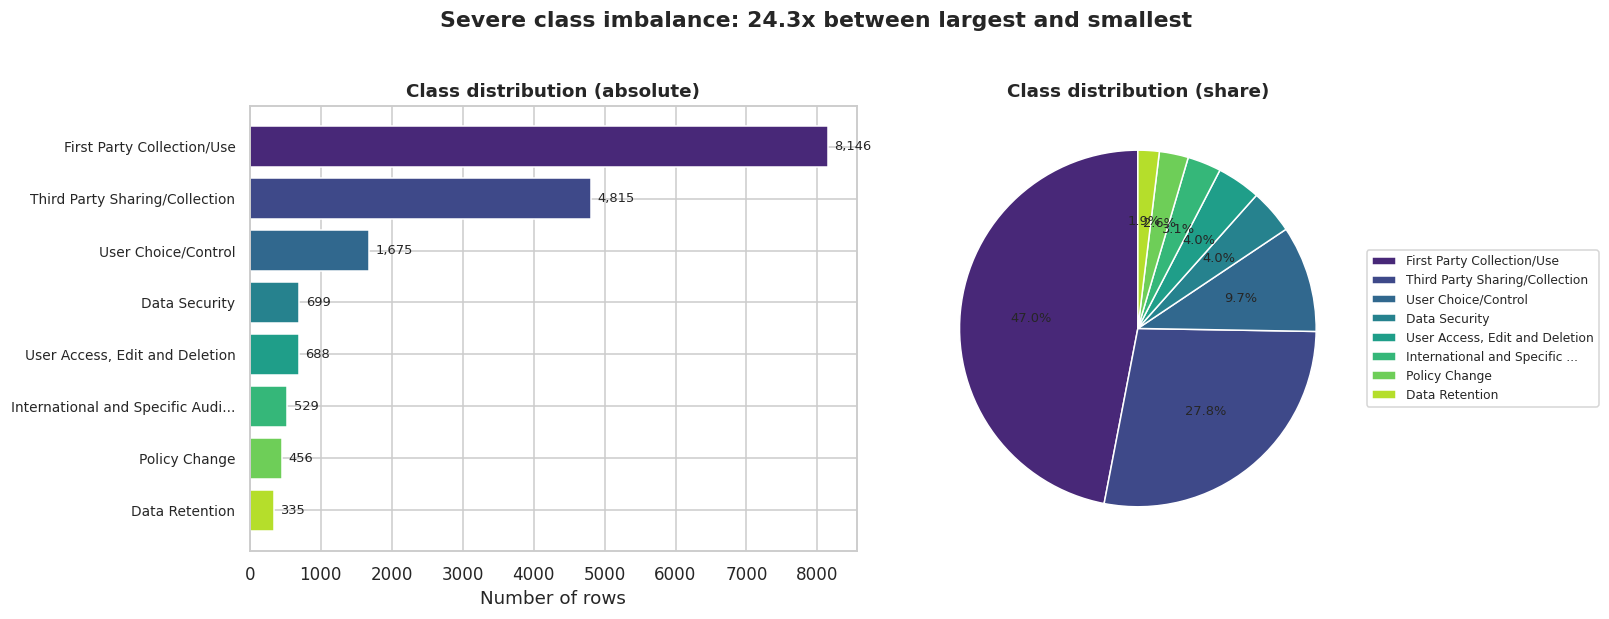
\includegraphics[width=0.95\columnwidth]{figures/class_distribution.png}
\caption{(a) Category distribution over 17,343 spans (24.3$\times$ largest/smallest ratio); (b) span length, clause length, and span length by category. Dashed lines mark the median.}
\label{fig:class_dist}
\end{figure}

\subsubsection{Multi-Practice Clauses}

1,119 of 3,204 distinct clauses (34.9\%) carry more than one category simultaneously. For example, a sentence such as ``we collect your email address and may share it with advertising partners unless you opt out'' simultaneously expresses First Party Collection/Use, Third Party Sharing/Collection, and User Choice/Control. This is why the clause is never used as the sole classification input; a clause-level single-label formulation would force one label onto text that legitimately expresses several practices.

\subsubsection{Boilerplate Reuse}

Under the conventional row-level random split, 113 of 115 policies appear on both sides and 95.2\% of test rows share clause text with some training row. Under the policy-disjoint split, that figure drops to 6.0\%---real-world boilerplate reuse across unrelated organizations rather than an artifact of the split.

\begin{figure}[t]
\centering
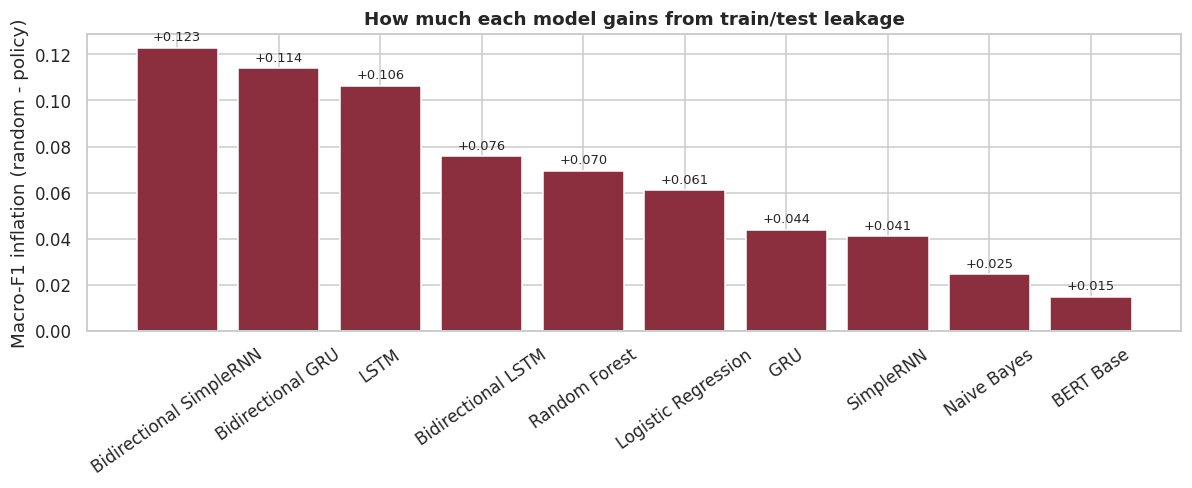
\includegraphics[width=0.95\columnwidth]{figures/leakage_inflation.png}
\caption{Left: percentage of test rows sharing clause text with training, by split scheme. Right: test-set class composition under each scheme. The two schemes differ not only in overlap but also in which policies compose the test set.}
\label{fig:leakage}
\end{figure}

This 95.2\% versus 6.0\% difference is the concrete motivation for the dual-scheme evaluation protocol.

\subsection{Preprocessing}

We define five preprocessing variants, each matched to a different downstream representation, as shown in Table~\ref{tab:preprocess}. Every variant first strips HTML markup and replaces URLs and email addresses with placeholder tokens ([URL], [EMAIL]). In the executed pipeline, the base variant was applied to both classical and recurrent models; minimal was applied to BERT Base.

\begin{table}[t]
\centering
\small
\begin{tabularx}{\columnwidth}{@{}p{1.9cm}XX@{}}
\toprule
\textbf{Variant} & \textbf{Processing} & \textbf{Intended For} \\
\midrule
base & HTML removal, placeholders, lower-case & Classical, RNN (actual) \\
no\_stopwords & base + NLTK stopword removal & Alt. TF-IDF \\
lemmatized & base + WordNet lemmatization & RNN (designed) \\
aggressive & stopwords + lemmatization & Sparse configs \\
minimal & HTML removal, lower-case only & BERT Base \\
\bottomrule
\end{tabularx}
\caption{Preprocessing variants and their intended usage.}
\label{tab:preprocess}
\end{table}

Figure~\ref{fig:preprocess} shows vocabulary size and mean span length for each variant. Stopword removal and lemmatization each reduce vocabulary by roughly one-third relative to base; combining both (aggressive) gives the smallest vocabulary.

\begin{figure}[t]
\centering
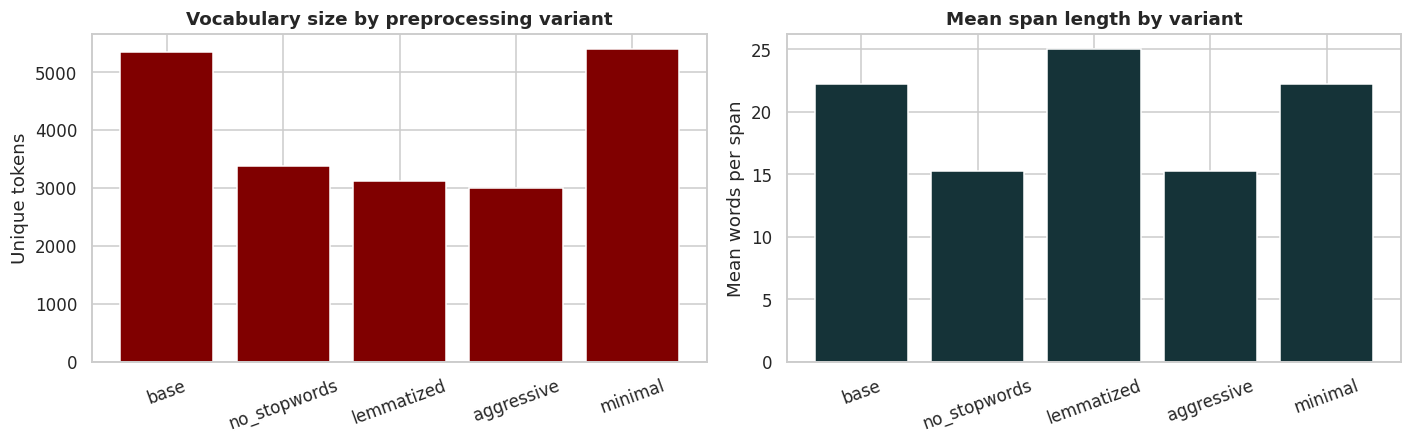
\includegraphics[width=0.95\columnwidth]{figures/preprocessing_variants.png}
\caption{Vocabulary size and mean span length for each preprocessing variant, measured on a 3,000-span sample. Stopword removal and lemmatization each reduce vocabulary by roughly a third relative to base.}
\label{fig:preprocess}
\end{figure}

\subsection{Word Representations}

\subsubsection{TF-IDF (Fully Evaluated)}

We use a 5,000-term vocabulary with unigrams and bigrams, minimum document frequency 5, maximum document frequency 0.8, and sublinear term-frequency scaling~\cite{pedregosa-etal-2011-scikit}. The vectorizer is refit independently on the training portion of each split scheme to prevent vocabulary leakage.

\subsubsection{Word2Vec (Implemented but Not Evaluated)}

A skip-gram Word2Vec pipeline was implemented using 100-dimensional embeddings, a context window of 5, and minimum token count of 2~\cite{mikolov-etal-2013-efficient}, via Gensim~\cite{rehurek-sojka-2010-software}. However, the Word2Vec pipeline was not executed for completed downstream classification experiment, so no Word2Vec classification results are reported.

\subsubsection{GloVe}

GloVe~\cite{pennington-etal-2014-glove} was not implemented in the executed notebook.

\subsection{Model Architectures and Hyperparameter Grids}

Table~\ref{tab:models} summarizes all ten models, their representations, and the configurations tested. For every model and split scheme, model selection uses validation macro-F1 and only the winning configuration is scored on the held-out test set.

\begin{table*}[t]
\centering
\begin{tabular}{@{}llll@{}}
\toprule
\textbf{Model Family} & \textbf{Model} & \textbf{Representation} & \textbf{Configs} \\
\midrule
\multirow{3}{*}{Classical} & Logistic Regression & TF-IDF & 3 \\
 & Random Forest & TF-IDF & 3 \\
 & Naive Bayes & TF-IDF & 3 \\
\midrule
\multirow{6}{*}{Recurrent} & SimpleRNN & Embedding & 3 \\
 & GRU & Embedding & 3 \\
 & LSTM & Embedding & 3 \\
 & Bidirectional SimpleRNN & Embedding & 3 \\
 & Bidirectional GRU & Embedding & 3 \\
 & Bidirectional LSTM & Embedding & 3 \\
\midrule
Transformer & BERT Base & Frozen layers & 6 \\
\bottomrule
\end{tabular}
\caption{Model architectures and hyperparameter configurations (3 configs per model $\times$ 2 schemes = 60 configurations).}
\label{tab:models}
\end{table*}

All six recurrent models share the same design: an embedding layer initialized from scratch, a recurrent or bidirectional recurrent layer, dropout regularization, and a dense softmax head. Input sequences are word-index-encoded from a training-only vocabulary and padded or truncated to 48 tokens. Models are implemented in PyTorch~\cite{paszke-etal-2019-pytorch}; final experiments ran in a CUDA-enabled Python 3.13 environment. BERT Base is fine-tuned via the HuggingFace Transformers library~\cite{wolf-etal-2020-transformers} with token embeddings and first 10 of 12 encoder layers frozen, and input truncated to 64 tokens.

\subsection{Split Schemes}

\subsubsection{Random Split (Leaky Comparison)}

Rows are split 70/15/15 (train/val/test), stratified by category, with no regard for policy origin (12,140/2,601/2,602 rows; 113 of 115 policies appear in both train and test). Reported only as a point of comparison against the honest condition.

\subsubsection{Policy-Disjoint Split (Honest Evaluation)}

Policies, not rows, are the unit of assignment, built from the corpus's own 92/23 policy split (76/16/23 policies; 11,344/2,088/3,911 rows). No policy's rows appear in more than one split. This is the paper's generalization estimate and the scheme used for every model-selection decision.

\section{Results}

All ten models were trained and evaluated under both split schemes for a combined 60 logged tuning runs (18 classical, 36 recurrent, 6 BERT Base). All numbers are drawn directly from the executed project notebook.

\subsection{Model Comparison}

Table~\ref{tab:results} reports test-set performance under both schemes. Figure~\ref{fig:model_comp} visualizes the comparison.

\begin{table*}[t]
\centering
\small
\setlength{\tabcolsep}{3.5pt}
\begin{tabular}{@{}lccc@{\hspace{1em}}ccc@{}}
\toprule
 & \multicolumn{3}{c}{Random Split (Leaky)} & \multicolumn{3}{c}{Policy-Disjoint (Honest)} \\
\textbf{Model} & Accuracy & Macro-F1 & Weighted-F1 & Accuracy & Macro-F1 & Weighted-F1 \\
\midrule
BERT Base & 0.759 & 0.721 & 0.755 & 0.715 & \textbf{0.706} & 0.704 \\
Naive Bayes & 0.758 & 0.726 & 0.755 & 0.688 & \textbf{0.701} & 0.688 \\
Logistic Regression & 0.774 & 0.753 & 0.771 & 0.691 & 0.692 & 0.690 \\
Random Forest & 0.780 & 0.721 & 0.774 & 0.665 & 0.652 & 0.665 \\
Bidirectional LSTM & 0.667 & 0.652 & 0.664 & 0.618 & 0.640 & 0.617 \\
Bidirectional GRU & 0.606 & 0.600 & 0.605 & 0.561 & 0.599 & 0.561 \\
LSTM & 0.612 & 0.597 & 0.609 & 0.567 & 0.591 & 0.567 \\
GRU & 0.583 & 0.569 & 0.581 & 0.540 & 0.563 & 0.540 \\
Bidirectional SimpleRNN & 0.269 & 0.257 & 0.268 & 0.159 & 0.134 & 0.158 \\
SimpleRNN & 0.259 & 0.249 & 0.257 & 0.152 & 0.131 & 0.151 \\
\bottomrule
\end{tabular}
\caption{Test performance at each model's best validated configuration under both split schemes, ranked by macro-F1 under policy-disjoint evaluation.}
\label{tab:results}
\end{table*}

Under the honest, policy-disjoint scheme, BERT Base reaches the best overall macro-F1 (0.706), narrowly ahead of Naive Bayes (0.701)---a gap of 0.005 that should be read as a near-tie rather than a decisive win. Logistic Regression comes third (0.692). SimpleRNN is the worst model overall (macro-F1 0.131, barely above a majority-class-only baseline), and Random Forest is the weakest of the three classical models (0.652).

Under the leaky random scheme, the picture looks quite different: Logistic Regression appears to lead (0.753) and BERT falls to fourth, behind both Random Forest and Naive Bayes. A concrete instance of the accuracy trap appears within the classical models: Random Forest has the highest accuracy of all ten models under the leaky split (0.780) yet the lowest macro-F1 among the three classical models (0.721)---a pattern consistent with the model benefiting disproportionately from the majority class's repeated boilerplate phrasing.

\begin{figure}[t]
\centering
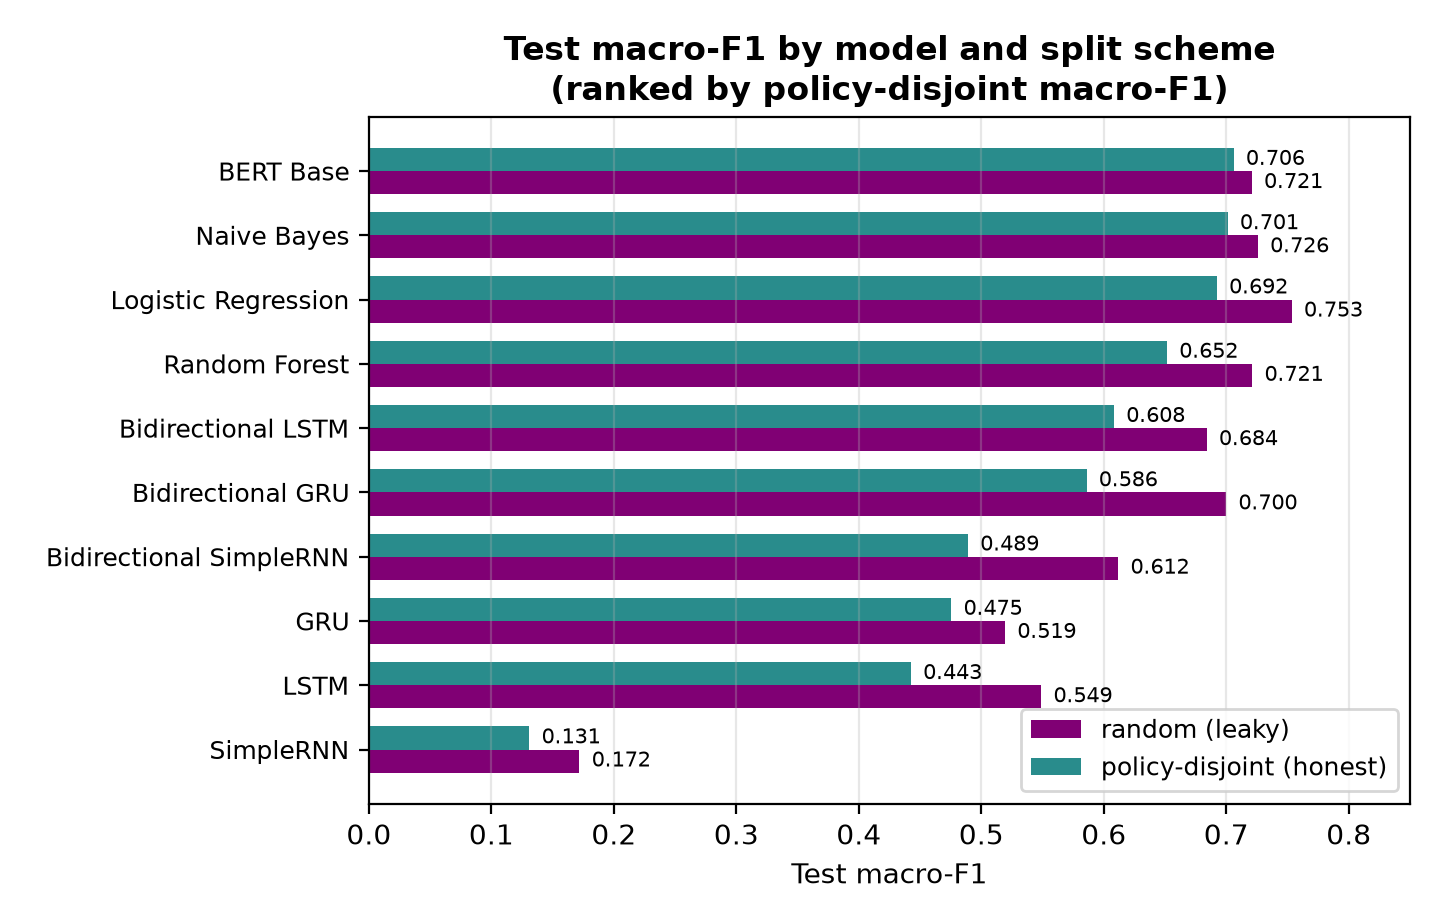
\includegraphics[width=0.95\columnwidth]{figures/model_comparison.png}
\caption{Macro-F1 comparison across all ten models under both split schemes.}
\label{fig:model_comp}
\end{figure}

\subsection{Evaluation-Protocol Gap Analysis}

\begin{figure}[t]
\centering
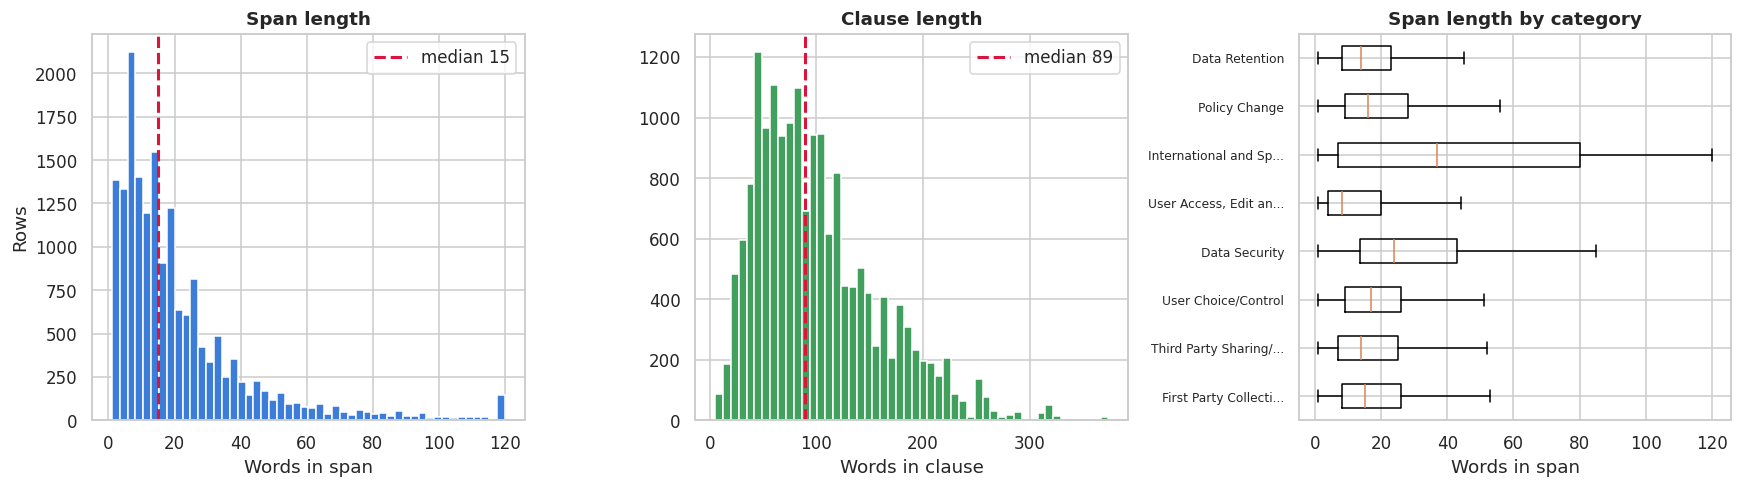
\includegraphics[width=0.95\columnwidth]{figures/span_length.png}
\caption{Evaluation-protocol macro-F1 gap (random-split score minus policy-disjoint score) by model; larger bars indicate models whose apparent performance depends more heavily on signal not available under honest evaluation.}
\label{fig:gap}
\end{figure}

The macro-F1 gap between the two schemes is shown in Figure~\ref{fig:gap}. We call this an evaluation-protocol gap rather than a pure measure of leakage because the two schemes also differ in test-set size and policy composition; the 95.2\% versus 6.0\% clause-overlap evidence makes leakage the most plausible dominant contributor.

The gap ranges from +0.015 (BERT Base) to +0.123 (Bidirectional SimpleRNN). The three classical models and BERT Base form a comparatively low-gap cluster (+0.015 to +0.070); the six recurrent architectures show both the largest and most variable gap (+0.041 to +0.123), with Bidirectional SimpleRNN, Bidirectional GRU, and unidirectional LSTM each exceeding +0.10.

BERT Base's gap of only +0.015 is consistent with the hypothesis that pretraining on a large external corpus reduces reliance on this dataset's own boilerplate.

\subsection{Per-Class Analysis}

\begin{table}[t]
\centering
\footnotesize
\setlength{\tabcolsep}{3pt}
\begin{tabularx}{\columnwidth}{@{}Xccc@{}}
\toprule
\textbf{Category} & \textbf{Precision} & \textbf{Recall} & \textbf{F1-Score} \\
\midrule
First Party Collection/Use & 0.82 & 0.73 & 0.77 \\
Third Party Sharing/Collection & 0.73 & 0.58 & 0.65 \\
User Choice/Control & 0.76 & 0.67 & 0.71 \\
Data Security & 0.68 & 0.62 & 0.65 \\
User Access & 0.88 & 0.74 & 0.80 \\
Edit and Deletion & 0.79 & 0.69 & 0.74 \\
International and Specific Audiences & 0.91 & 0.85 & 0.88 \\
Policy Change & 0.93 & 0.84 & 0.88 \\
Data Retention & 0.86 & 0.35 & 0.50 \\
\bottomrule
\end{tabularx}
\caption{Per-class P/R/F1 for BERT Base (policy-disjoint; accuracy 0.715, macro-F1 0.706).}
\label{tab:perclass}
\end{table}

Table~\ref{tab:perclass} reports per-class results for BERT Base under the policy-disjoint test set. The per-class results show no clear relationship between class frequency and classification performance: several relatively small categories achieve high F1 scores, whereas some much larger categories remain more difficult.

Policy Change and International and Specific Audiences are among the smallest categories yet score highest (F1 0.88), because both use distinctive formulaic vocabulary (``we may update this policy from time to time''; ``residents of the European Economic Area'') that a model learns from relatively few examples.

The dominant error mode is confusion between First Party Collection/Use and Third Party Sharing/Collection: both describe data collection and differ chiefly in who receives the data, a distinction sometimes carried by a single noun phrase within a short span.

Data Retention is the one category where scarcity appears to matter: precision is high (0.86) but recall is the lowest of any category (0.35), consistent with a model that recognizes the category when it commits to it but has too few training examples to do so reliably.

\begin{figure*}[t]
\centering
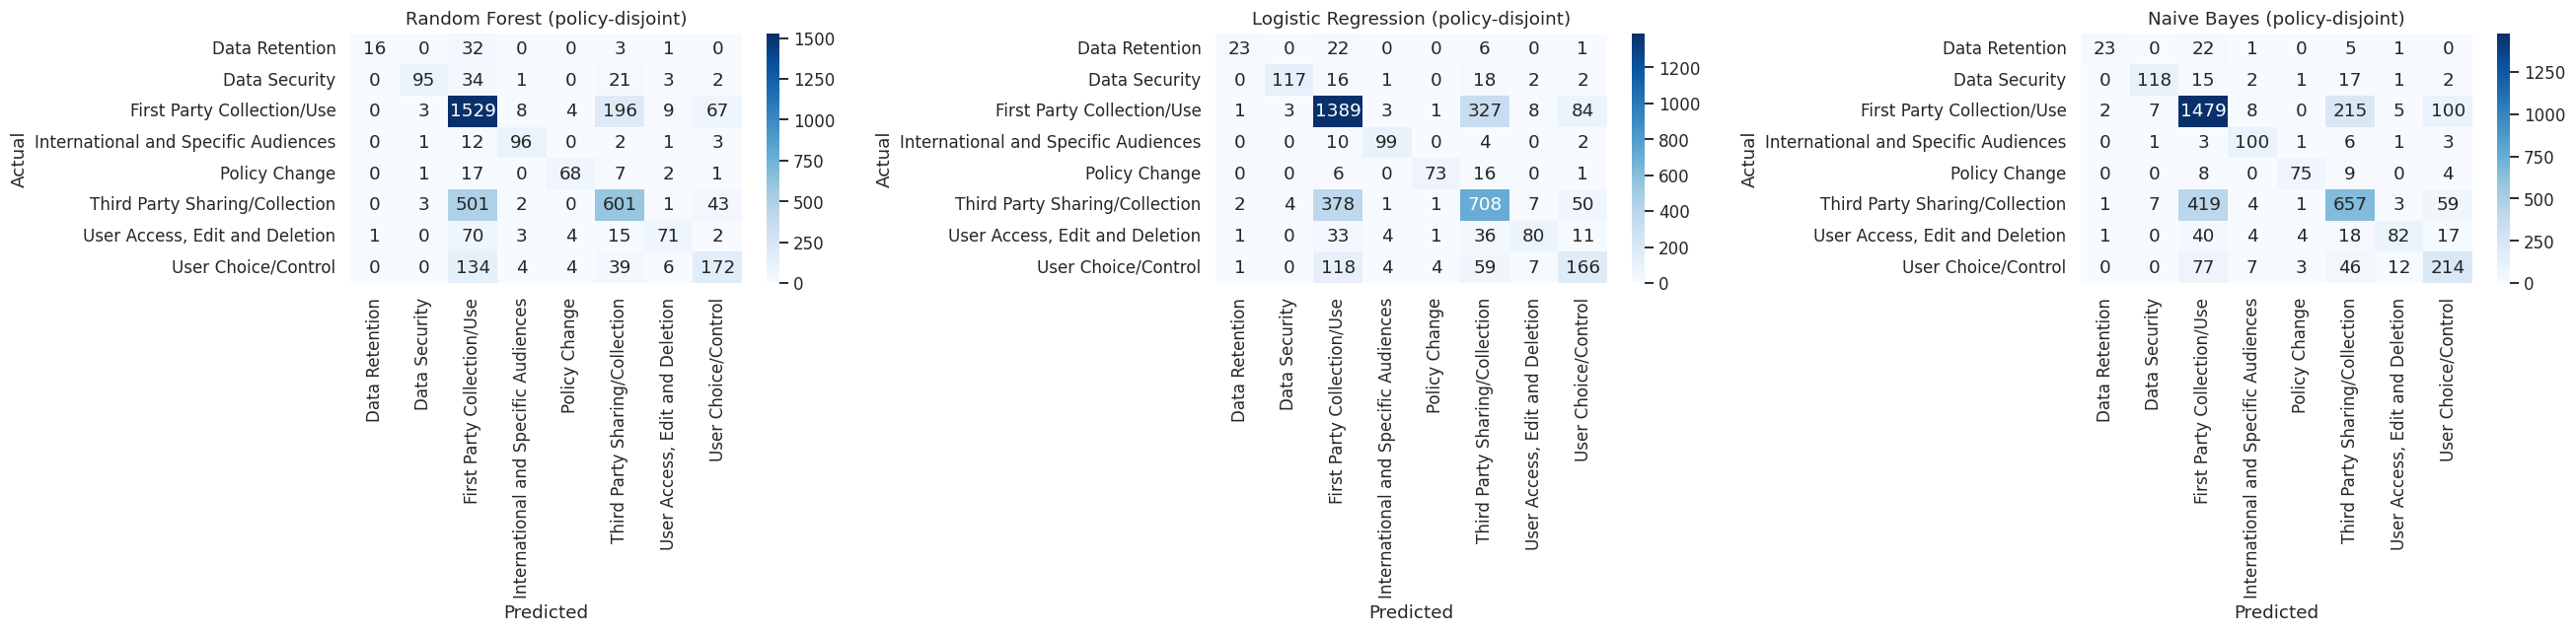
\includegraphics[width=\textwidth]{figures/confusion_matrices_classical.png}
\caption{Row-normalized confusion matrices for the three classical models on the policy-disjoint test set.}
\label{fig:confusion}
\end{figure*}

\subsection{Best and Worst Configurations}

Among the 60 tuning runs, the winning configuration for BERT Base under the policy-disjoint scheme is learning rate $3 \times 10^{-5}$, batch size 32 (validation macro-F1 0.723, test macro-F1 0.706). The winning classical configuration is Naive Bayes with $\alpha = 0.05$ (validation macro-F1 0.680, test macro-F1 0.701). The weakest configuration across all models is SimpleRNN with embed=128, hidden=64, dropout=0.3, $lr=10^{-3}$ under the policy scheme (validation macro-F1 0.110).

\subsection{Representation Status}

TF-IDF is the only representation with completed downstream classification; every classical model result in Table~\ref{tab:results} uses TF-IDF. The Word2Vec pipeline was implemented but not executed for completed downstream classification. GloVe was not implemented. BERT Base results come from partial, layer-frozen fine-tuning; no full fine-tune was attempted.

\section{Discussion and Findings}

Our central finding is that a conventional stratified split, scored on accuracy or on an unexamined single-split macro-F1, would have led to incorrect conclusions about model ranking. Several recurrent architectures would be ranked well above their honest positions, silently, with nothing in the leaky split's own numbers to flag the problem.

The document-level structure in privacy policies is extreme but not unique: contracts, regulatory filings, terms of service, and form letters all exhibit similar template reuse. Our findings suggest that any text classification task built on such documents should adopt document-grouped evaluation as standard practice.

\section{Conclusion}

We systematically compare evaluation protocols for privacy-practice classification across three classical, six recurrent, and one transformer model. Our key findings are:

\begin{enumerate}
\item Evaluating on a conventional row-level split changes not just the absolute numbers but which model appears to win (RQ1).
\item The evaluation-protocol gap is largest for recurrent architectures trained from scratch and smallest for BERT Base and classical models (RQ2).
\item Under honest, policy-disjoint evaluation, BERT Base leads at macro-F1 0.706, narrowly ahead of Naive Bayes (0.701); the classical models' competitiveness suggests that privacy-practice categories carry strong lexical cues that TF-IDF captures effectively on short spans (RQ3).
\end{enumerate}

We take the leakage-versus-honest contrast as evidence that document-grouped evaluation should be standard practice.

\section{Limitations}

The six recurrent models process every padded position in a 48-token sequence without length masking; short spans continue being processed through trailing padding, which may partly explain the recurrent family's large evaluation-protocol gap. The executed pipeline applied base preprocessing to the recurrent models rather than the designed lemmatized variant; the isolated effect is untested. Random seeds are not reset per configuration inside the recurrent tuning loop. Only TF-IDF downstream classification is complete; Word2Vec was not evaluated and GloVe was not implemented. BERT results come from partial, layer-frozen fine-tuning rather than a full fine-tune. All results are oracle-span: a deployed system would additionally need an upstream span-detection step.

\section{Future Work}

The most pressing fixes are:
\begin{enumerate}
\item Retrain the six recurrent models with length-aware packing and per-configuration seed resets.
\item Complete the Word2Vec downstream evaluation.
\item Apply the designed lemmatized preprocessing to recurrent models to isolate its effect.
\item Feed span-plus-clause context to specifically help the First Party versus Third Party confusion.
\item Implement minority-class-aware training strategies for Data Retention.
\item Execute a full, non-frozen BERT fine-tune given GPU access.
\end{enumerate}

\section*{Acknowledgments}

This work was conducted as part of the CSE440 course project at BRAC University. We thank the annotators of the OPP-115 corpus and the maintainers of the datasets and libraries used in this research.

\bibliography{custom}
\bibliographystyle{plainnat}

\end{document}
